\documentclass[twoside]{book}

% Packages required by doxygen
\usepackage{fixltx2e}
\usepackage{calc}
\usepackage{doxygen}
\usepackage[export]{adjustbox} % also loads graphicx
\usepackage{graphicx}
\usepackage[utf8]{inputenc}
\usepackage{makeidx}
\usepackage{multicol}
\usepackage{multirow}
\PassOptionsToPackage{warn}{textcomp}
\usepackage{textcomp}
\usepackage[nointegrals]{wasysym}
\usepackage[table]{xcolor}

% NLS support packages
\usepackage{polski}
\usepackage[T1]{fontenc}

% Font selection
\usepackage[T1]{fontenc}
\usepackage[scaled=.90]{helvet}
\usepackage{courier}
\usepackage{amssymb}
\usepackage{sectsty}
\renewcommand{\familydefault}{\sfdefault}
\allsectionsfont{%
  \fontseries{bc}\selectfont%
  \color{darkgray}%
}
\renewcommand{\DoxyLabelFont}{%
  \fontseries{bc}\selectfont%
  \color{darkgray}%
}
\newcommand{\+}{\discretionary{\mbox{\scriptsize$\hookleftarrow$}}{}{}}

% Page & text layout
\usepackage{geometry}
\geometry{%
  a4paper,%
  top=2.5cm,%
  bottom=2.5cm,%
  left=2.5cm,%
  right=2.5cm%
}
\tolerance=750
\hfuzz=15pt
\hbadness=750
\setlength{\emergencystretch}{15pt}
\setlength{\parindent}{0cm}
\setlength{\parskip}{3ex plus 2ex minus 2ex}
\makeatletter
\renewcommand{\paragraph}{%
  \@startsection{paragraph}{4}{0ex}{-1.0ex}{1.0ex}{%
    \normalfont\normalsize\bfseries\SS@parafont%
  }%
}
\renewcommand{\subparagraph}{%
  \@startsection{subparagraph}{5}{0ex}{-1.0ex}{1.0ex}{%
    \normalfont\normalsize\bfseries\SS@subparafont%
  }%
}
\makeatother

% Headers & footers
\usepackage{fancyhdr}
\pagestyle{fancyplain}
\fancyhead[LE]{\fancyplain{}{\bfseries\thepage}}
\fancyhead[CE]{\fancyplain{}{}}
\fancyhead[RE]{\fancyplain{}{\bfseries\leftmark}}
\fancyhead[LO]{\fancyplain{}{\bfseries\rightmark}}
\fancyhead[CO]{\fancyplain{}{}}
\fancyhead[RO]{\fancyplain{}{\bfseries\thepage}}
\fancyfoot[LE]{\fancyplain{}{}}
\fancyfoot[CE]{\fancyplain{}{}}
\fancyfoot[RE]{\fancyplain{}{\bfseries\scriptsize Wygenerowano przez Doxygen }}
\fancyfoot[LO]{\fancyplain{}{\bfseries\scriptsize Wygenerowano przez Doxygen }}
\fancyfoot[CO]{\fancyplain{}{}}
\fancyfoot[RO]{\fancyplain{}{}}
\renewcommand{\footrulewidth}{0.4pt}
\renewcommand{\chaptermark}[1]{%
  \markboth{#1}{}%
}
\renewcommand{\sectionmark}[1]{%
  \markright{\thesection\ #1}%
}

% Indices & bibliography
\usepackage{natbib}
\usepackage[titles]{tocloft}
\setcounter{tocdepth}{3}
\setcounter{secnumdepth}{5}
\makeindex

% Hyperlinks (required, but should be loaded last)
\usepackage{ifpdf}
\ifpdf
  \usepackage[pdftex,pagebackref=true]{hyperref}
\else
  \usepackage[ps2pdf,pagebackref=true]{hyperref}
\fi
\hypersetup{%
  colorlinks=true,%
  linkcolor=blue,%
  citecolor=blue,%
  unicode%
}

% Custom commands
\newcommand{\clearemptydoublepage}{%
  \newpage{\pagestyle{empty}\cleardoublepage}%
}

\usepackage{caption}
\captionsetup{labelsep=space,justification=centering,font={bf},singlelinecheck=off,skip=4pt,position=top}

%===== C O N T E N T S =====

\begin{document}

% Titlepage & ToC
\hypersetup{pageanchor=false,
             bookmarksnumbered=true,
             pdfencoding=unicode
            }
\pagenumbering{roman}
\begin{titlepage}
\vspace*{7cm}
\begin{center}%
{\Large Epidemia }\\
\vspace*{1cm}
{\large Wygenerowano przez Doxygen 1.8.11}\\
\end{center}
\end{titlepage}
\clearemptydoublepage
\tableofcontents
\clearemptydoublepage
\pagenumbering{arabic}
\hypersetup{pageanchor=true}

%--- Begin generated contents ---
\chapter{Projekt-\/\+Epidemia}
\label{md_README}
\hypertarget{md_README}{}
\input{md_README}
\chapter{Indeks hierarchiczny}
\section{Hierarchia klas}
Ta lista dziedziczenia posortowana jest z grubsza, choć nie całkowicie, alfabetycznie\+:\begin{DoxyCompactList}
\item \contentsline{section}{Country}{\pageref{classCountry}}{}
\item \contentsline{section}{Disease}{\pageref{classDisease}}{}
\begin{DoxyCompactList}
\item \contentsline{section}{Common\+Disease}{\pageref{classCommonDisease}}{}
\item \contentsline{section}{Mutagen}{\pageref{classMutagen}}{}
\item \contentsline{section}{Ultra\+Vegan}{\pageref{classUltraVegan}}{}
\end{DoxyCompactList}
\item \contentsline{section}{Person}{\pageref{classPerson}}{}
\begin{DoxyCompactList}
\item \contentsline{section}{Common\+Person}{\pageref{classCommonPerson}}{}
\begin{DoxyCompactList}
\item \contentsline{section}{Scientist}{\pageref{classScientist}}{}
\end{DoxyCompactList}
\item \contentsline{section}{Vegan}{\pageref{classVegan}}{}
\end{DoxyCompactList}
\end{DoxyCompactList}

\chapter{Indeks klas}
\section{Lista klas}
Tutaj znajdują się klasy, struktury, unie i interfejsy wraz z ich krótkimi opisami\+:\begin{DoxyCompactList}
\item\contentsline{section}{\hyperlink{classCommonDisease}{Common\+Disease} }{\pageref{classCommonDisease}}{}
\item\contentsline{section}{\hyperlink{classCommonPerson}{Common\+Person} }{\pageref{classCommonPerson}}{}
\item\contentsline{section}{\hyperlink{classCountry}{Country} }{\pageref{classCountry}}{}
\item\contentsline{section}{\hyperlink{classDisease}{Disease} }{\pageref{classDisease}}{}
\item\contentsline{section}{\hyperlink{classMutagen}{Mutagen} }{\pageref{classMutagen}}{}
\item\contentsline{section}{\hyperlink{classPerson}{Person} }{\pageref{classPerson}}{}
\item\contentsline{section}{\hyperlink{classScientist}{Scientist} }{\pageref{classScientist}}{}
\item\contentsline{section}{\hyperlink{classUltraVegan}{Ultra\+Vegan} }{\pageref{classUltraVegan}}{}
\item\contentsline{section}{\hyperlink{classVegan}{Vegan} }{\pageref{classVegan}}{}
\end{DoxyCompactList}

\chapter{Dokumentacja klas}
\hypertarget{classCommonDisease}{}\section{Dokumentacja klasy Common\+Disease}
\label{classCommonDisease}\index{Common\+Disease@{Common\+Disease}}
Diagram dziedziczenia dla Common\+Disease\begin{figure}[H]
\begin{center}
\leavevmode
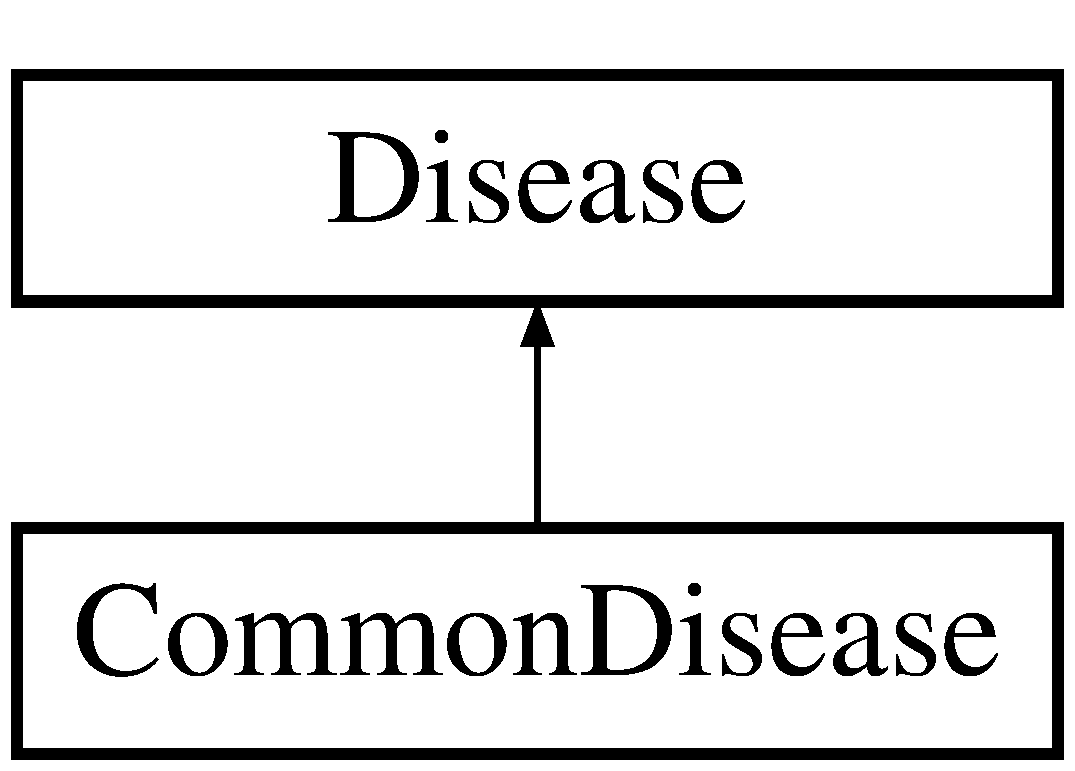
\includegraphics[height=2.000000cm]{classCommonDisease}
\end{center}
\end{figure}
\subsection*{Metody publiczne}
\begin{DoxyCompactItemize}
\item 
int {\bfseries attack\+Chance} ()\hypertarget{classCommonDisease_aedc0c61d8adb52f672f7d8ad4fb92087}{}\label{classCommonDisease_aedc0c61d8adb52f672f7d8ad4fb92087}

\item 
virtual int {\bfseries who} ()\hypertarget{classCommonDisease_a740853d832994e8a5b64410049113fe6}{}\label{classCommonDisease_a740853d832994e8a5b64410049113fe6}

\item 
virtual bool {\bfseries try\+Attack} ()\hypertarget{classCommonDisease_a628842276e544539a55ab484a9bb7bce}{}\label{classCommonDisease_a628842276e544539a55ab484a9bb7bce}

\item 
virtual string {\bfseries description} ()\hypertarget{classCommonDisease_a1804255e2d381189f1dfa398c62001ec}{}\label{classCommonDisease_a1804255e2d381189f1dfa398c62001ec}

\end{DoxyCompactItemize}


Dokumentacja dla tej klasy została wygenerowana z plików\+:\begin{DoxyCompactItemize}
\item 
Disease.\+h\item 
Disease.\+cpp\end{DoxyCompactItemize}

\hypertarget{classCommonPerson}{}\section{Dokumentacja klasy Common\+Person}
\label{classCommonPerson}\index{Common\+Person@{Common\+Person}}
Diagram dziedziczenia dla Common\+Person\begin{figure}[H]
\begin{center}
\leavevmode
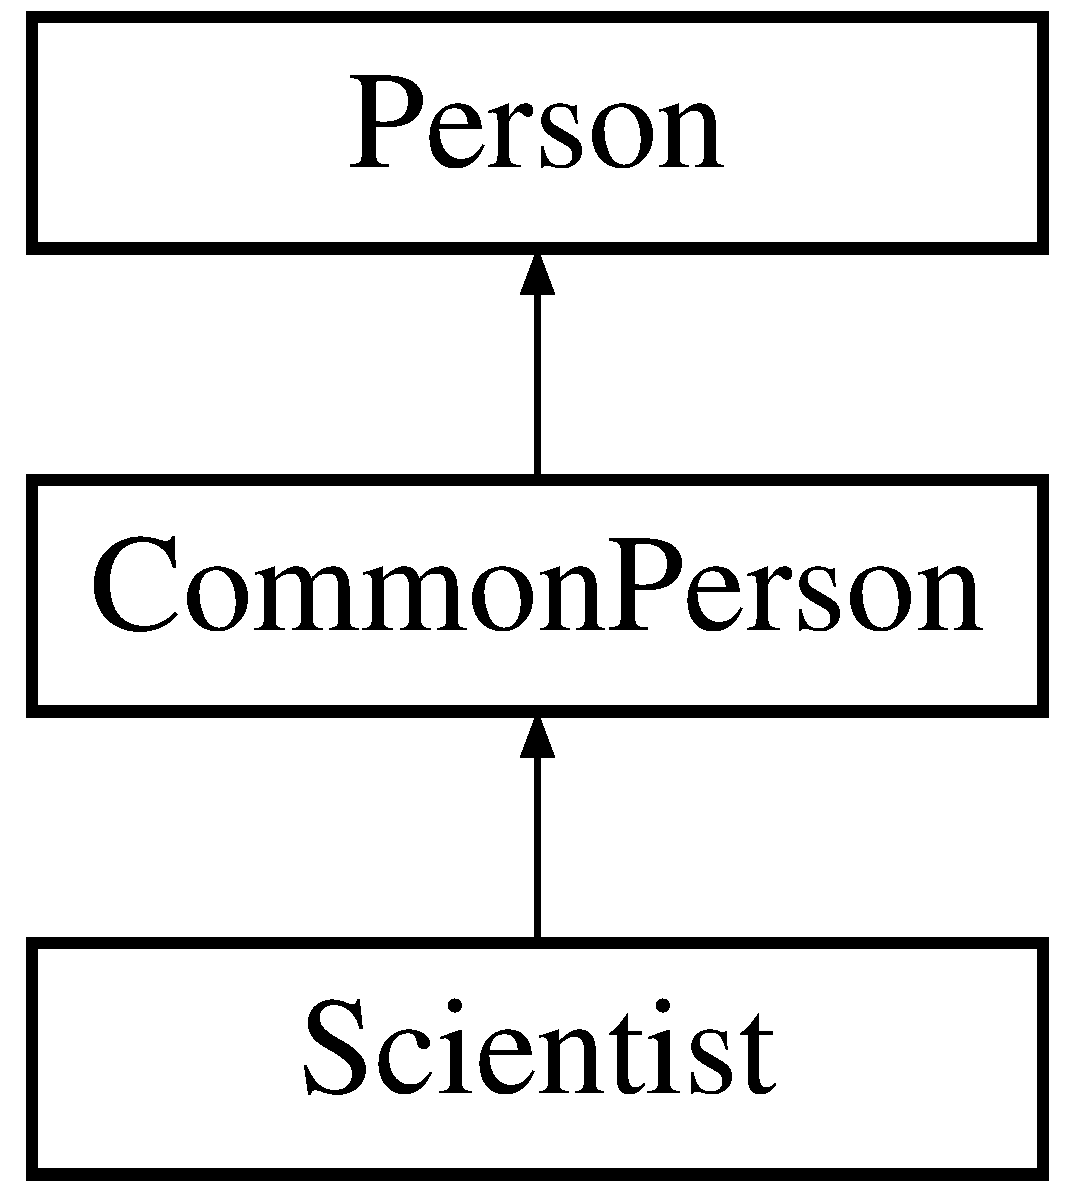
\includegraphics[height=3.000000cm]{classCommonPerson}
\end{center}
\end{figure}
\subsection*{Metody publiczne}
\begin{DoxyCompactItemize}
\item 
int \hyperlink{classCommonPerson_aa6124a1a40f875cb3d739dee53af1724}{attack} ()
\item 
int \hyperlink{classCommonPerson_a1334a830f0d44df46ea92cd7ef2ebc29}{attack\+Chance} ()
\item 
int \hyperlink{classCommonPerson_a8de900c43b59c0c14e896d4cba68cb76}{dodge\+Chance} ()
\item 
int \hyperlink{classCommonPerson_acf2a1d582a17534ea43da4e51cde5b3b}{intelligence} ()
\item 
virtual int \hyperlink{classCommonPerson_af0b8d634f112c3f9d564124700758c6f}{who} ()
\item 
virtual string \hyperlink{classCommonPerson_a50960e537f0353dbd8bee7a53b7963e3}{description} ()
\end{DoxyCompactItemize}


\subsection{Dokumentacja funkcji składowych}
\index{Common\+Person@{Common\+Person}!attack@{attack}}
\index{attack@{attack}!Common\+Person@{Common\+Person}}
\subsubsection[{\texorpdfstring{attack()}{attack()}}]{\setlength{\rightskip}{0pt plus 5cm}int Common\+Person\+::attack (
\begin{DoxyParamCaption}
{}
\end{DoxyParamCaption}
)\hspace{0.3cm}{\ttfamily [inline]}, {\ttfamily [virtual]}}\hypertarget{classCommonPerson_aa6124a1a40f875cb3d739dee53af1724}{}\label{classCommonPerson_aa6124a1a40f875cb3d739dee53af1724}
$\ast$\+Zadaje dmg osobom. 

Implementuje \hyperlink{classPerson_a7cabe13a0c3122fa7ac0e9f005a87346}{Person}.

\index{Common\+Person@{Common\+Person}!attack\+Chance@{attack\+Chance}}
\index{attack\+Chance@{attack\+Chance}!Common\+Person@{Common\+Person}}
\subsubsection[{\texorpdfstring{attack\+Chance()}{attackChance()}}]{\setlength{\rightskip}{0pt plus 5cm}int Common\+Person\+::attack\+Chance (
\begin{DoxyParamCaption}
{}
\end{DoxyParamCaption}
)\hspace{0.3cm}{\ttfamily [inline]}, {\ttfamily [virtual]}}\hypertarget{classCommonPerson_a1334a830f0d44df46ea92cd7ef2ebc29}{}\label{classCommonPerson_a1334a830f0d44df46ea92cd7ef2ebc29}
$\ast$\+Atak wyprowadzany przez osobę 

Implementuje \hyperlink{classPerson_a4f525256f6ffb3135e61bd22ff48c37a}{Person}.

\index{Common\+Person@{Common\+Person}!description@{description}}
\index{description@{description}!Common\+Person@{Common\+Person}}
\subsubsection[{\texorpdfstring{description()}{description()}}]{\setlength{\rightskip}{0pt plus 5cm}string Common\+Person\+::description (
\begin{DoxyParamCaption}
{}
\end{DoxyParamCaption}
)\hspace{0.3cm}{\ttfamily [virtual]}}\hypertarget{classCommonPerson_a50960e537f0353dbd8bee7a53b7963e3}{}\label{classCommonPerson_a50960e537f0353dbd8bee7a53b7963e3}
$\ast$0-\/\+Common 1-\/\+Scientist 2-\/\+Vegans 

Implementuje \hyperlink{classPerson_aef5de94dd30ff791097a0c1444999e60}{Person}.



Reimplementowana w \hyperlink{classScientist_a31ff8bf82c31257c1a22e16fcca3da7b}{Scientist}.

\index{Common\+Person@{Common\+Person}!dodge\+Chance@{dodge\+Chance}}
\index{dodge\+Chance@{dodge\+Chance}!Common\+Person@{Common\+Person}}
\subsubsection[{\texorpdfstring{dodge\+Chance()}{dodgeChance()}}]{\setlength{\rightskip}{0pt plus 5cm}int Common\+Person\+::dodge\+Chance (
\begin{DoxyParamCaption}
{}
\end{DoxyParamCaption}
)\hspace{0.3cm}{\ttfamily [inline]}, {\ttfamily [virtual]}}\hypertarget{classCommonPerson_a8de900c43b59c0c14e896d4cba68cb76}{}\label{classCommonPerson_a8de900c43b59c0c14e896d4cba68cb76}
$\ast$\+Szansa na atak 

Implementuje \hyperlink{classPerson_adb64abc2cc5e02f1ebbc7823e7921168}{Person}.

\index{Common\+Person@{Common\+Person}!intelligence@{intelligence}}
\index{intelligence@{intelligence}!Common\+Person@{Common\+Person}}
\subsubsection[{\texorpdfstring{intelligence()}{intelligence()}}]{\setlength{\rightskip}{0pt plus 5cm}int Common\+Person\+::intelligence (
\begin{DoxyParamCaption}
{}
\end{DoxyParamCaption}
)\hspace{0.3cm}{\ttfamily [inline]}, {\ttfamily [virtual]}}\hypertarget{classCommonPerson_acf2a1d582a17534ea43da4e51cde5b3b}{}\label{classCommonPerson_acf2a1d582a17534ea43da4e51cde5b3b}
$\ast$\+Szansa na unik 

Implementuje \hyperlink{classPerson_a3d18aad60b7ea1305e1a469d7d5fc216}{Person}.



Reimplementowana w \hyperlink{classScientist_a5a8cd2cea36347764ad85328a814c892}{Scientist}.

\index{Common\+Person@{Common\+Person}!who@{who}}
\index{who@{who}!Common\+Person@{Common\+Person}}
\subsubsection[{\texorpdfstring{who()}{who()}}]{\setlength{\rightskip}{0pt plus 5cm}virtual int Common\+Person\+::who (
\begin{DoxyParamCaption}
{}
\end{DoxyParamCaption}
)\hspace{0.3cm}{\ttfamily [inline]}, {\ttfamily [virtual]}}\hypertarget{classCommonPerson_af0b8d634f112c3f9d564124700758c6f}{}\label{classCommonPerson_af0b8d634f112c3f9d564124700758c6f}
$\ast$\+Inteligencja 

Implementuje \hyperlink{classPerson_a7d102d6c8ed786f4ad1fcd2c3cea2f3e}{Person}.



Reimplementowana w \hyperlink{classScientist_a8ae5a60d92adca7fa1840ffe369e12ba}{Scientist}.



Dokumentacja dla tej klasy została wygenerowana z plików\+:\begin{DoxyCompactItemize}
\item 
Person.\+h\item 
Person.\+cpp\end{DoxyCompactItemize}

\hypertarget{classCountry}{}\section{Dokumentacja klasy Country}
\label{classCountry}\index{Country@{Country}}
\subsection*{Metody publiczne}
\begin{DoxyCompactItemize}
\item 
{\bfseries Country} (unsigned int population, int sl, int vl, int zl)\hypertarget{classCountry_afc0bccd7503b1878f47d816aad1be547}{}\label{classCountry_afc0bccd7503b1878f47d816aad1be547}

\item 
int {\bfseries persons} ()\hypertarget{classCountry_ab1dd10f4a0d9d1cf53fb8a9f4079de93}{}\label{classCountry_ab1dd10f4a0d9d1cf53fb8a9f4079de93}

\item 
int {\bfseries infected\+Persons} ()\hypertarget{classCountry_a3b8ee891f42aed5f438e564df7bf3b0a}{}\label{classCountry_a3b8ee891f42aed5f438e564df7bf3b0a}

\item 
int {\bfseries cure} ()\hypertarget{classCountry_a464c5b103990dfab70b50217edb60876}{}\label{classCountry_a464c5b103990dfab70b50217edb60876}

\item 
void {\bfseries Infect\+Person} (std\+::vector$<$ \hyperlink{classPerson}{Person} $\ast$ $>$\+::iterator person\+Opponent)\hypertarget{classCountry_a5c46c5155c99175ffb3acef946312be0}{}\label{classCountry_a5c46c5155c99175ffb3acef946312be0}

\item 
void {\bfseries fight} (fstream \&output, int output\+Info)\hypertarget{classCountry_ae7333fae8f953c2f39da1a46c3d3862a}{}\label{classCountry_ae7333fae8f953c2f39da1a46c3d3862a}

\item 
void {\bfseries spread\+Virus} (int i, fstream \&output)\hypertarget{classCountry_aa8fe23fc3002c75b93946cae54c4f202}{}\label{classCountry_aa8fe23fc3002c75b93946cae54c4f202}

\item 
bool {\bfseries search\+For\+Cure} (fstream \&output)\hypertarget{classCountry_aceb291a044a495483951745eecece744}{}\label{classCountry_aceb291a044a495483951745eecece744}

\item 
void {\bfseries cure\+Some\+Infected\+Persons} (fstream \&output)\hypertarget{classCountry_a87a885d659d7e47e405d5d445fd4f0ee}{}\label{classCountry_a87a885d659d7e47e405d5d445fd4f0ee}

\item 
string {\bfseries description} ()\hypertarget{classCountry_a15d7e9b23f141f837fec76cedd76683b}{}\label{classCountry_a15d7e9b23f141f837fec76cedd76683b}

\item 
string {\bfseries show\+Everyone} ()\hypertarget{classCountry_a167fa855a40dd3bb0274ee8c01c994c8}{}\label{classCountry_a167fa855a40dd3bb0274ee8c01c994c8}

\end{DoxyCompactItemize}


Dokumentacja dla tej klasy została wygenerowana z plików\+:\begin{DoxyCompactItemize}
\item 
Country.\+h\item 
Country.\+cpp\end{DoxyCompactItemize}

\hypertarget{classDisease}{}\section{Dokumentacja klasy Disease}
\label{classDisease}\index{Disease@{Disease}}
Diagram dziedziczenia dla Disease\begin{figure}[H]
\begin{center}
\leavevmode
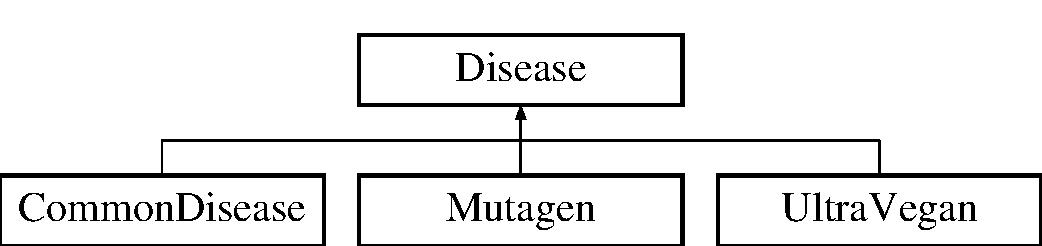
\includegraphics[height=2.000000cm]{classDisease}
\end{center}
\end{figure}
\subsection*{Metody publiczne}
\begin{DoxyCompactItemize}
\item 
int {\bfseries disease\+ID} ()\hypertarget{classDisease_aa767f0483110104290041bddc272fdbb}{}\label{classDisease_aa767f0483110104290041bddc272fdbb}

\item 
int {\bfseries disease\+HP} ()\hypertarget{classDisease_af9f0bf00f479ca6ecafcaa1d4664631a}{}\label{classDisease_af9f0bf00f479ca6ecafcaa1d4664631a}

\item 
void {\bfseries damage} (int dmg)\hypertarget{classDisease_a8e453ce6d51ac090aada3bf7993d04d9}{}\label{classDisease_a8e453ce6d51ac090aada3bf7993d04d9}

\item 
bool {\bfseries is\+Dead} ()\hypertarget{classDisease_aec6c5373af8923c7eeb23ab8601298cb}{}\label{classDisease_aec6c5373af8923c7eeb23ab8601298cb}

\item 
virtual int {\bfseries attack\+Chance} ()=0\hypertarget{classDisease_ae527ac8784e17279f5b796f83c0374d4}{}\label{classDisease_ae527ac8784e17279f5b796f83c0374d4}

\item 
virtual int {\bfseries who} ()=0\hypertarget{classDisease_a08e55daa6094568570d869ac86fa1f3b}{}\label{classDisease_a08e55daa6094568570d869ac86fa1f3b}

\item 
virtual bool {\bfseries try\+Attack} ()=0\hypertarget{classDisease_a4186b72a74f3d2e654b38254ca0d32b7}{}\label{classDisease_a4186b72a74f3d2e654b38254ca0d32b7}

\item 
virtual string {\bfseries description} ()=0\hypertarget{classDisease_ab472fecd75428fa29567021314ff6bbe}{}\label{classDisease_ab472fecd75428fa29567021314ff6bbe}

\end{DoxyCompactItemize}


Dokumentacja dla tej klasy została wygenerowana z plików\+:\begin{DoxyCompactItemize}
\item 
Disease.\+h\item 
main.\+cpp\end{DoxyCompactItemize}

\hypertarget{classMutagen}{}\section{Dokumentacja klasy Mutagen}
\label{classMutagen}\index{Mutagen@{Mutagen}}
Diagram dziedziczenia dla Mutagen\begin{figure}[H]
\begin{center}
\leavevmode
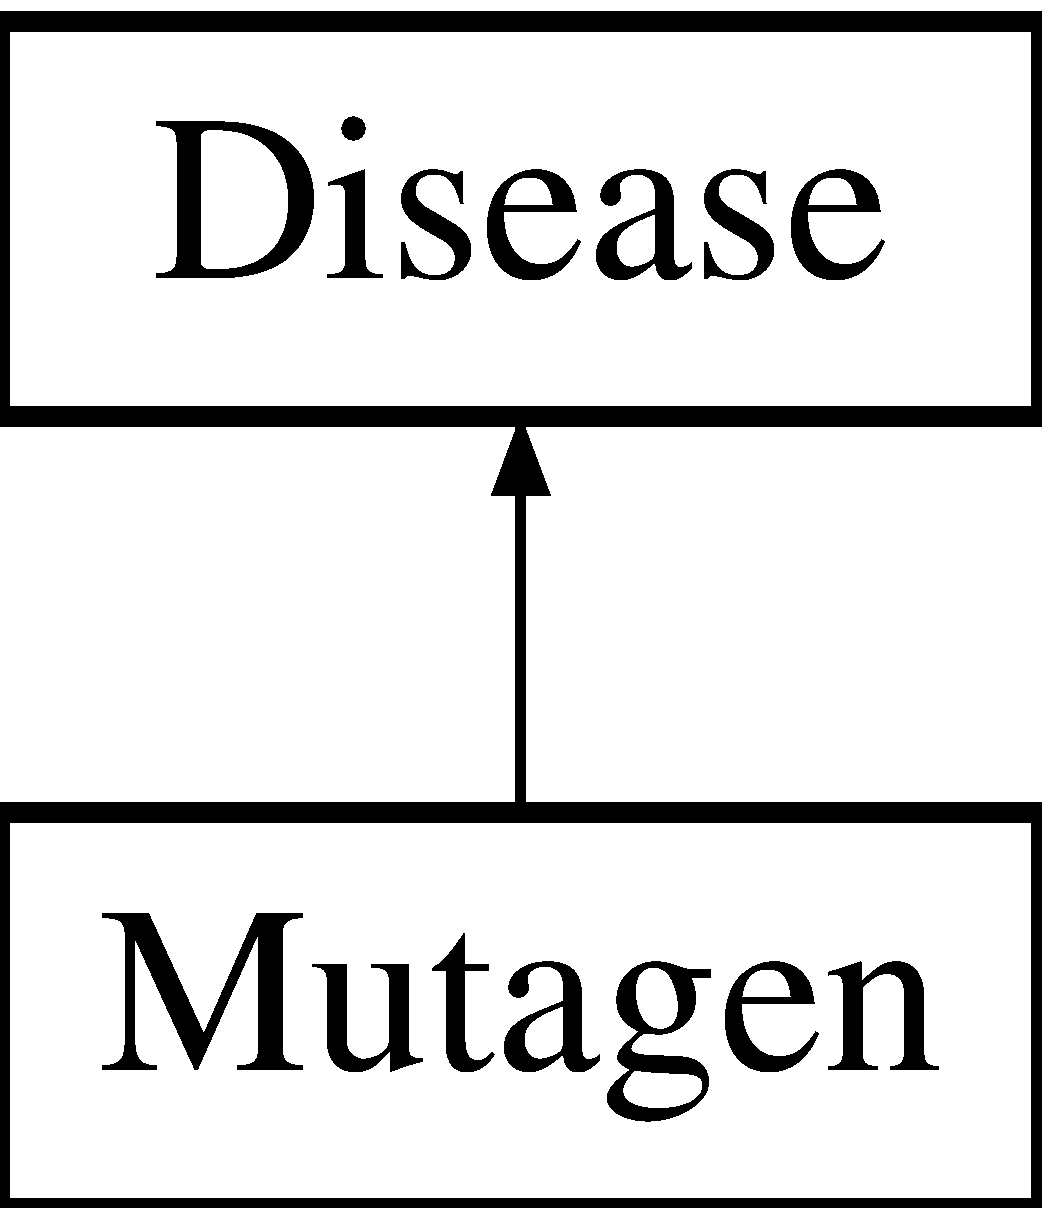
\includegraphics[height=2.000000cm]{classMutagen}
\end{center}
\end{figure}
\subsection*{Metody publiczne}
\begin{DoxyCompactItemize}
\item 
int {\bfseries attack\+Chance} ()\hypertarget{classMutagen_afcd518c374fa5802575bcc5b4e7b98cd}{}\label{classMutagen_afcd518c374fa5802575bcc5b4e7b98cd}

\item 
int {\bfseries attack\+Count} ()\hypertarget{classMutagen_a2049d82c471219087055da1bc4bb6f71}{}\label{classMutagen_a2049d82c471219087055da1bc4bb6f71}

\item 
virtual int {\bfseries who} ()\hypertarget{classMutagen_a620c593682e56b1a0039f8f1aeea4f39}{}\label{classMutagen_a620c593682e56b1a0039f8f1aeea4f39}

\item 
virtual bool {\bfseries try\+Attack} ()\hypertarget{classMutagen_a6c495ef43212c37e125b771d8d02898c}{}\label{classMutagen_a6c495ef43212c37e125b771d8d02898c}

\item 
virtual string {\bfseries description} ()\hypertarget{classMutagen_a47ac6ab84065448d49954c57fb555a3e}{}\label{classMutagen_a47ac6ab84065448d49954c57fb555a3e}

\end{DoxyCompactItemize}


Dokumentacja dla tej klasy została wygenerowana z plików\+:\begin{DoxyCompactItemize}
\item 
Disease.\+h\item 
Disease.\+cpp\end{DoxyCompactItemize}

\hypertarget{classPerson}{}\section{Dokumentacja klasy Person}
\label{classPerson}\index{Person@{Person}}
Diagram dziedziczenia dla Person\begin{figure}[H]
\begin{center}
\leavevmode
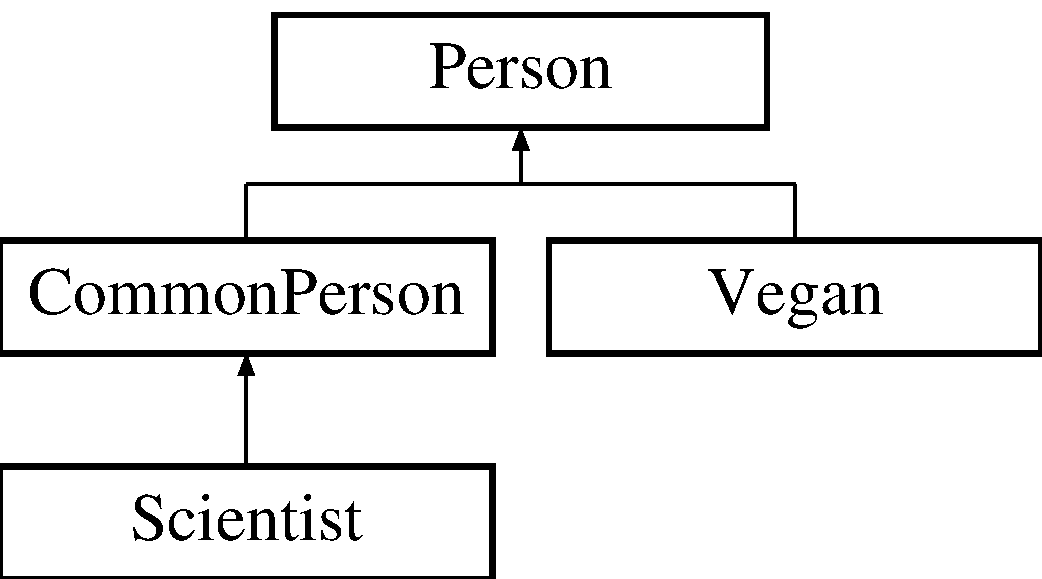
\includegraphics[height=3.000000cm]{classPerson}
\end{center}
\end{figure}
\subsection*{Metody publiczne}
\begin{DoxyCompactItemize}
\item 
int {\bfseries person\+ID} ()\hypertarget{classPerson_a4ea656fa93595281740221a37e223044}{}\label{classPerson_a4ea656fa93595281740221a37e223044}

\item 
int {\bfseries person\+HP} ()\hypertarget{classPerson_a3054b34b9ecdc924630f54f6a8b7bc02}{}\label{classPerson_a3054b34b9ecdc924630f54f6a8b7bc02}

\item 
int {\bfseries is\+Dead} ()\hypertarget{classPerson_a4d88afde6fa07378dbdb18eb50ab9e64}{}\label{classPerson_a4d88afde6fa07378dbdb18eb50ab9e64}

\item 
void {\bfseries damage} (int dmg)\hypertarget{classPerson_a5dbdaa48f3456c30c792fb40cf16b9eb}{}\label{classPerson_a5dbdaa48f3456c30c792fb40cf16b9eb}

\item 
virtual int {\bfseries attack} ()=0\hypertarget{classPerson_a7cabe13a0c3122fa7ac0e9f005a87346}{}\label{classPerson_a7cabe13a0c3122fa7ac0e9f005a87346}

\item 
virtual int {\bfseries attack\+Chance} ()=0\hypertarget{classPerson_a4f525256f6ffb3135e61bd22ff48c37a}{}\label{classPerson_a4f525256f6ffb3135e61bd22ff48c37a}

\item 
virtual int {\bfseries dodge\+Chance} ()=0\hypertarget{classPerson_adb64abc2cc5e02f1ebbc7823e7921168}{}\label{classPerson_adb64abc2cc5e02f1ebbc7823e7921168}

\item 
virtual int {\bfseries intelligence} ()=0\hypertarget{classPerson_a3d18aad60b7ea1305e1a469d7d5fc216}{}\label{classPerson_a3d18aad60b7ea1305e1a469d7d5fc216}

\item 
virtual int {\bfseries who} ()=0\hypertarget{classPerson_a7d102d6c8ed786f4ad1fcd2c3cea2f3e}{}\label{classPerson_a7d102d6c8ed786f4ad1fcd2c3cea2f3e}

\item 
virtual string {\bfseries description} ()=0\hypertarget{classPerson_aef5de94dd30ff791097a0c1444999e60}{}\label{classPerson_aef5de94dd30ff791097a0c1444999e60}

\end{DoxyCompactItemize}


Dokumentacja dla tej klasy została wygenerowana z plików\+:\begin{DoxyCompactItemize}
\item 
Person.\+h\item 
main.\+cpp\end{DoxyCompactItemize}

\hypertarget{classScientist}{}\section{Dokumentacja klasy Scientist}
\label{classScientist}\index{Scientist@{Scientist}}
Diagram dziedziczenia dla Scientist\begin{figure}[H]
\begin{center}
\leavevmode
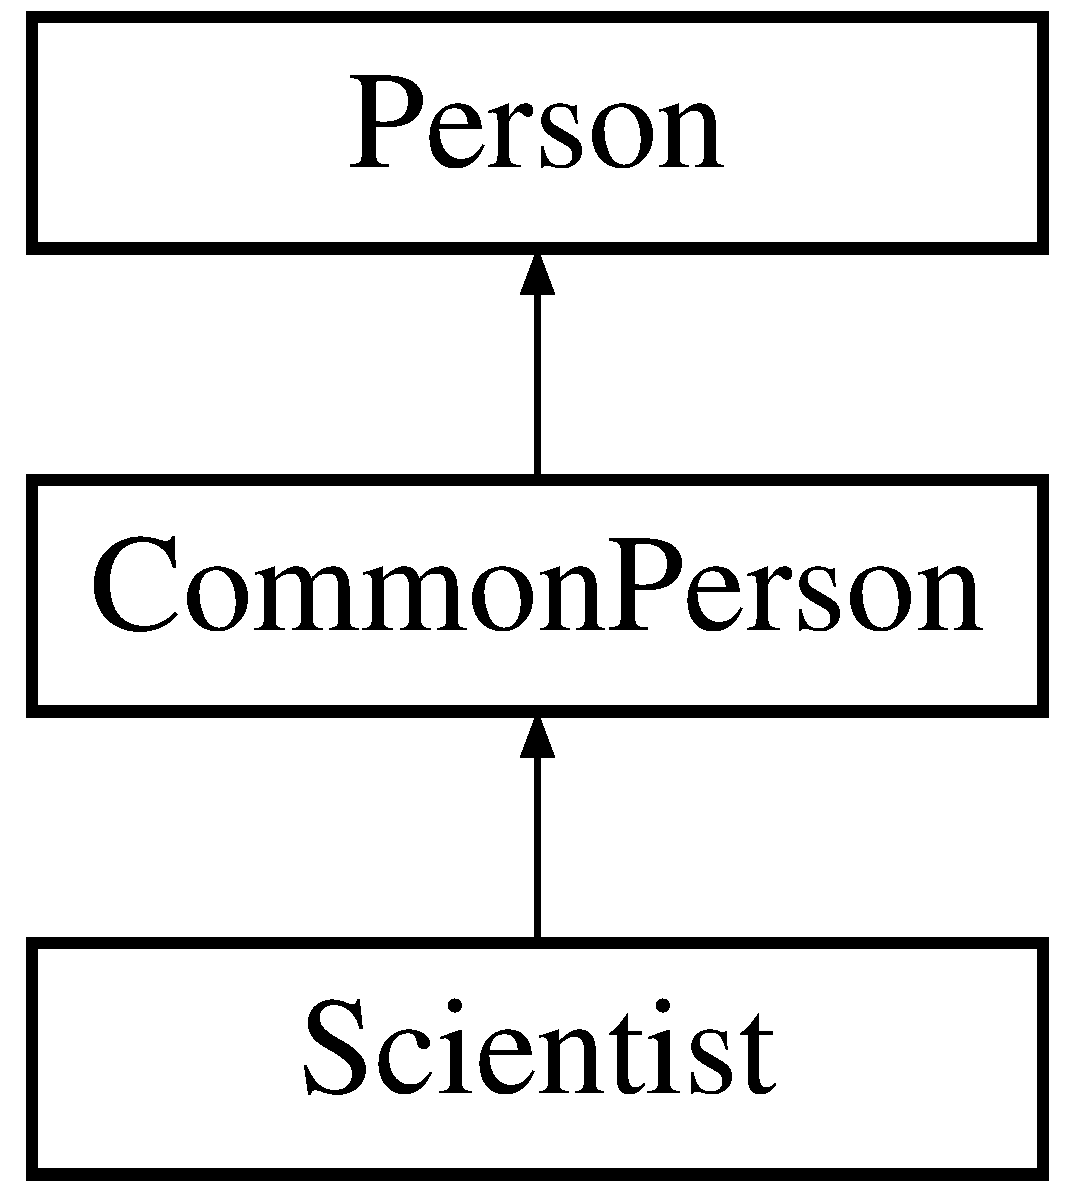
\includegraphics[height=3.000000cm]{classScientist}
\end{center}
\end{figure}
\subsection*{Metody publiczne}
\begin{DoxyCompactItemize}
\item 
int {\bfseries intelligence} ()\hypertarget{classScientist_a5a8cd2cea36347764ad85328a814c892}{}\label{classScientist_a5a8cd2cea36347764ad85328a814c892}

\item 
virtual int {\bfseries who} ()\hypertarget{classScientist_a8ae5a60d92adca7fa1840ffe369e12ba}{}\label{classScientist_a8ae5a60d92adca7fa1840ffe369e12ba}

\item 
virtual string {\bfseries description} ()\hypertarget{classScientist_a31ff8bf82c31257c1a22e16fcca3da7b}{}\label{classScientist_a31ff8bf82c31257c1a22e16fcca3da7b}

\end{DoxyCompactItemize}


Dokumentacja dla tej klasy została wygenerowana z plików\+:\begin{DoxyCompactItemize}
\item 
Person.\+h\item 
Person.\+cpp\end{DoxyCompactItemize}

\hypertarget{classUltraVegan}{}\section{Dokumentacja klasy Ultra\+Vegan}
\label{classUltraVegan}\index{Ultra\+Vegan@{Ultra\+Vegan}}
Diagram dziedziczenia dla Ultra\+Vegan\begin{figure}[H]
\begin{center}
\leavevmode
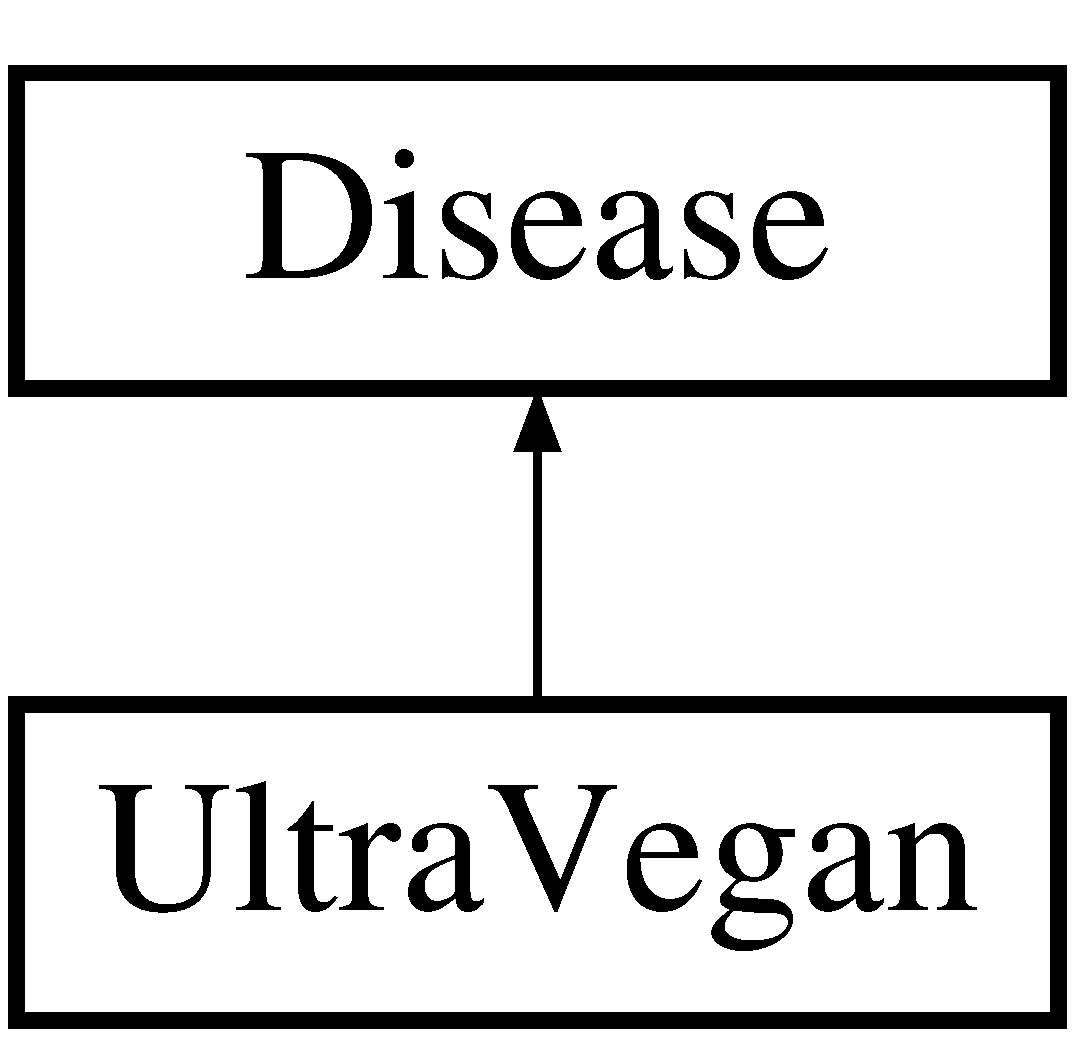
\includegraphics[height=2.000000cm]{classUltraVegan}
\end{center}
\end{figure}
\subsection*{Metody publiczne}
\begin{DoxyCompactItemize}
\item 
int {\bfseries attack\+Chance} ()\hypertarget{classUltraVegan_a84155389c92f4fc624722d31cd2e400f}{}\label{classUltraVegan_a84155389c92f4fc624722d31cd2e400f}

\item 
virtual int {\bfseries who} ()\hypertarget{classUltraVegan_a25c49b013633a9e9e1e8fb6a9f103f3f}{}\label{classUltraVegan_a25c49b013633a9e9e1e8fb6a9f103f3f}

\item 
virtual bool {\bfseries try\+Attack} ()\hypertarget{classUltraVegan_a40927f8fbccf4c87f0ce72b1bcd459a3}{}\label{classUltraVegan_a40927f8fbccf4c87f0ce72b1bcd459a3}

\item 
virtual string {\bfseries description} ()\hypertarget{classUltraVegan_a429d15dd51cf97460bbac469b4159998}{}\label{classUltraVegan_a429d15dd51cf97460bbac469b4159998}

\end{DoxyCompactItemize}


Dokumentacja dla tej klasy została wygenerowana z plików\+:\begin{DoxyCompactItemize}
\item 
Disease.\+h\item 
Disease.\+cpp\end{DoxyCompactItemize}

\hypertarget{classVegan}{}\section{Dokumentacja klasy Vegan}
\label{classVegan}\index{Vegan@{Vegan}}
Diagram dziedziczenia dla Vegan\begin{figure}[H]
\begin{center}
\leavevmode
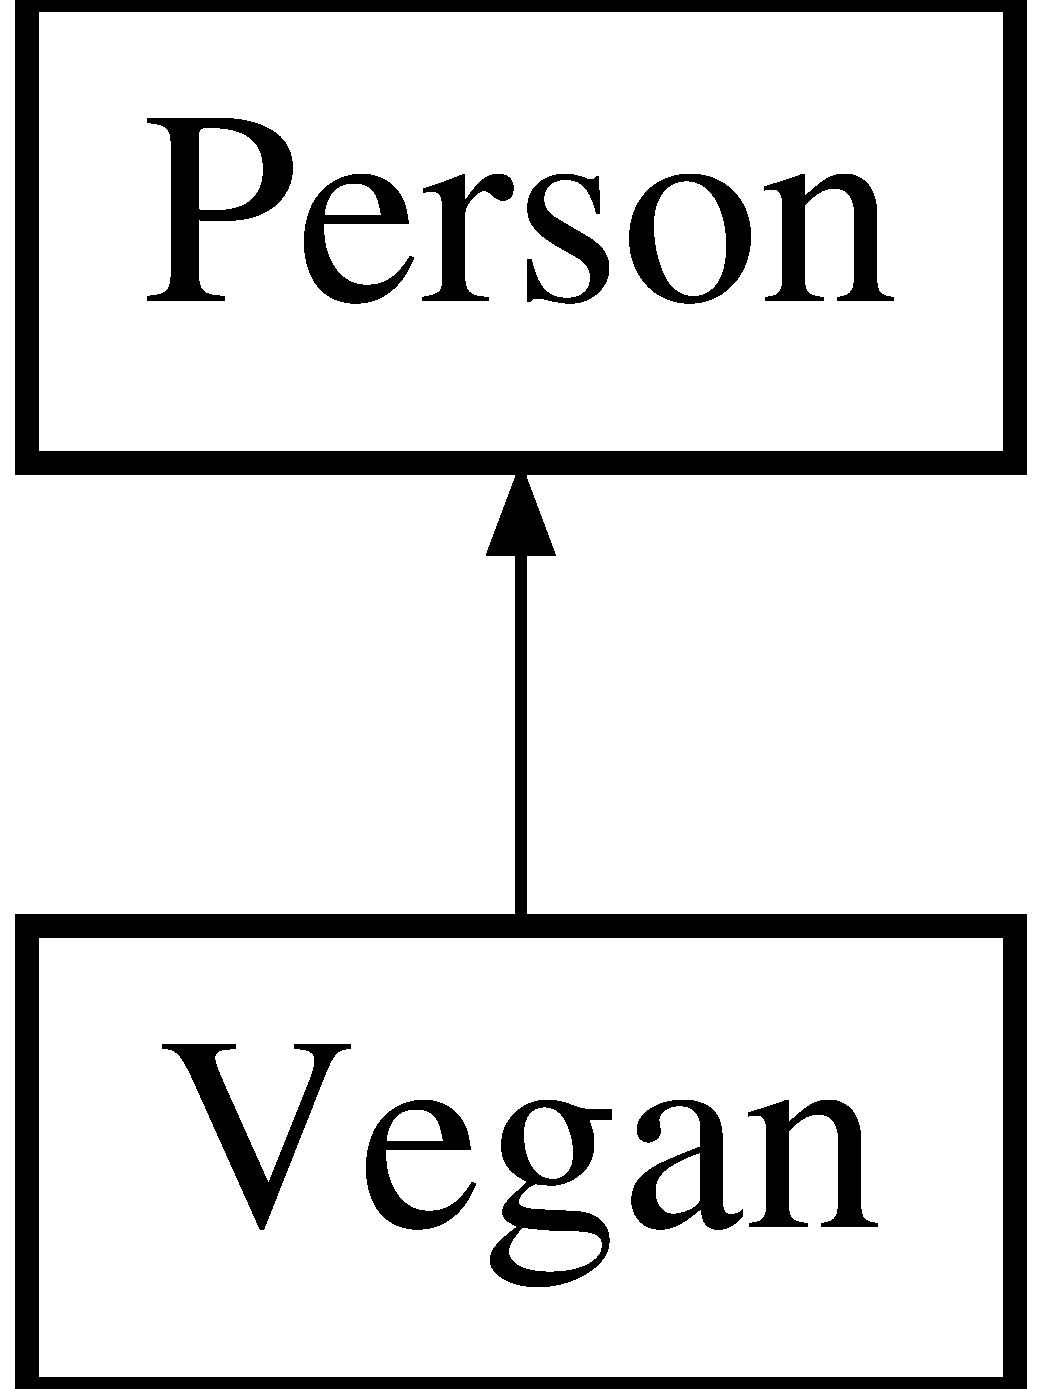
\includegraphics[height=2.000000cm]{classVegan}
\end{center}
\end{figure}
\subsection*{Metody publiczne}
\begin{DoxyCompactItemize}
\item 
int {\bfseries attack} ()\hypertarget{classVegan_a49da538a7bdc7cf95e2995d374844690}{}\label{classVegan_a49da538a7bdc7cf95e2995d374844690}

\item 
int {\bfseries attack\+Chance} ()\hypertarget{classVegan_add22eca62b8e3c3ffe93da1d0e5d91f5}{}\label{classVegan_add22eca62b8e3c3ffe93da1d0e5d91f5}

\item 
int {\bfseries dodge\+Chance} ()\hypertarget{classVegan_aad321fbb0951c24515900f002ede0286}{}\label{classVegan_aad321fbb0951c24515900f002ede0286}

\item 
int {\bfseries intelligence} ()\hypertarget{classVegan_a2b63e0fcdefc296e4164d4e26fda4aa8}{}\label{classVegan_a2b63e0fcdefc296e4164d4e26fda4aa8}

\item 
virtual int {\bfseries who} ()\hypertarget{classVegan_a46b4008d435a0ab8c0986ceda995d2da}{}\label{classVegan_a46b4008d435a0ab8c0986ceda995d2da}

\item 
virtual string {\bfseries description} ()\hypertarget{classVegan_a021955c46ba7952ab46a07a768f9b3b3}{}\label{classVegan_a021955c46ba7952ab46a07a768f9b3b3}

\end{DoxyCompactItemize}


Dokumentacja dla tej klasy została wygenerowana z plików\+:\begin{DoxyCompactItemize}
\item 
Person.\+h\item 
Person.\+cpp\end{DoxyCompactItemize}

%--- End generated contents ---

% Index
\backmatter
\newpage
\phantomsection
\clearemptydoublepage
\addcontentsline{toc}{chapter}{Indeks}
\printindex

\end{document}
